% Ubah judul dan label berikut sesuai dengan yang diinginkan.
\section{Architecture}
\label{sec:arsitektur}
The system developed is divided into three parts. The first part is the FrontEnd part, used for displaying the website. This part is built with Next.js, a React framework for building websites. The second part is the machine learnign back end, which runs the LLM model to answer user queries. This component is created using Python and FastAPI. It is separated from the back end that responsible for data presentation and authentication management because the LLM model requires significant resources and takes a long time to run. This separation aims to prevent the server from becoming inaccessible while the LLM model is running. The third part is the management back end part for data presentation and authentication management, developed with Node.js and Express.js. This part serves the data needed by the FrontEnd and manages user authentication. It also handles conversation history and stores it in MongoDB. The system configuration can be seen in Figure \ref*{fig:system}.

\begin{figure*}
  \centering
  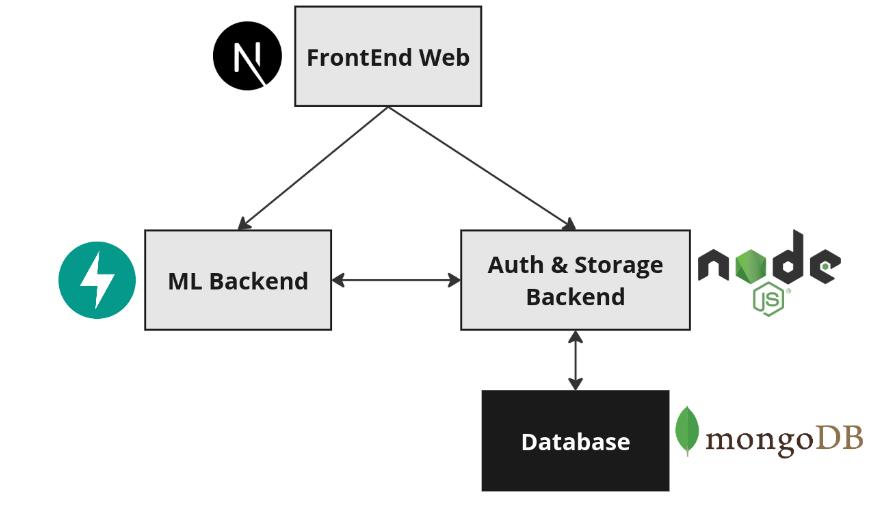
\includegraphics[width=.6\textwidth]{gambar/struktur-sistem.jpg}
  \caption{System structure}
  \label{fig:system}
\end{figure*}

% Ubah paragraf-paragraf pada bagian ini sesuai dengan yang diinginkan.
The further explanation is as follows.
\subsection{Front End}
\label{subsec:frontend}

The first part of the system is implemented by creating the website interface using Next.js and utilizing ShadCn as a UI library. Next.js, known for its robust features for server-side rendering and static site generation, provides a solid foundation for building high-performance web applications. ShadCn, as a UI library, offers a collection of pre-designed components that enhance the visual appeal and usability of the website. The interface is designed to be simple, prioritizing functionality over complexity. This simplicity ensures that users can easily navigate the site and access its features without confusion. The main feature of the website is the chat functionality, which is prominently displayed to facilitate user interaction. The chat interface is intuitive, allowing users to quickly engage in conversations with the system.

In addition to the chat feature, there are buttons for Login and SignUp, ensuring secure access to the website's services. Every time a user accesses the website, they must log in. This login process is essential for retrieving the user's conversation data, ensuring that each user can continue their interactions seamlessly from where they left off. Whenever a user engages in a conversation, the website forwards the conversation data to the BackEnd that handles the LLM (Large Language Model) model. This BackEnd is responsible for processing the user's queries and generating appropriate responses. After receiving a response from the LLM model, the website displays the response to the user in the chat interface. While the website is preparing the response, the user is unable to send additional messages. This temporary restriction is implemented to prevent excessive requests that could overwhelm the system and degrade performance. By managing the flow of requests in this manner, the system ensures that each response is processed efficiently and delivered to the user without unnecessary delays.


\subsection{RAG Back End}
\label{subsec:RAG}

This part of the back end system handle LLM model to answer user queries. Before using data for the language model, it is necessary to search for relevant data. To perform this data search, searches are conducted by looking at the location of the data within the vector. For this, data must be converted into a vector format that can be computed. There are many methods for doing this, such as \emph{one-hot}, \emph{Word2Vec}, and \emph{Doc2Vec}. These methods provide effective pathways for text quantification but often ignore contextual information. The \emph{Transformer} model, introduced by Google in 2017, overcomes the shortcomings of existing text quantification methods and is built using unsupervised training on large volumes of unlabeled corpus data \cite{vaswani2017attention}. The \emph{Transformer} is a neural network architecture widely used in NLP, text classification, question-answering systems, and more. This model consists of several \emph{encoders} and \emph{decoders}, each composed of several layers of identical blocks. These blocks are stacked together to form the overall \emph{Transformer} architecture \cite{miao2016processing}. The structure of the \emph{transformer} can be seen in Figure \ref*{fig:transformer}.

\begin{figure*}
  \centering
  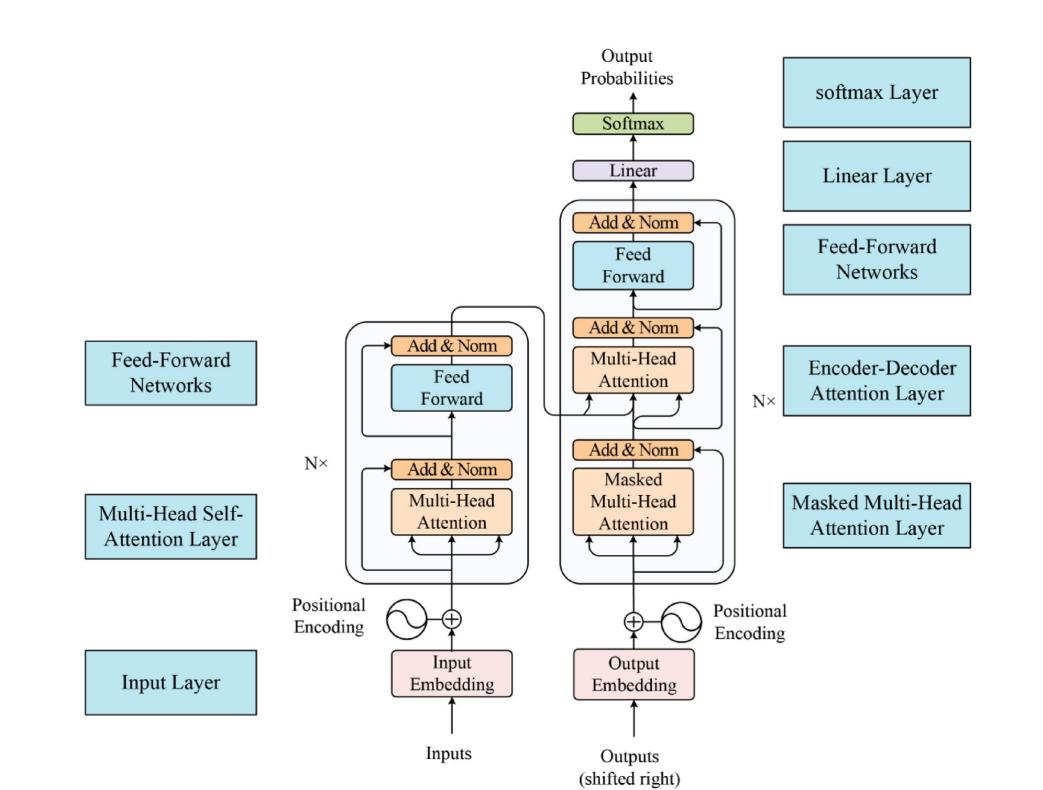
\includegraphics[width=.7\textwidth]{gambar/struktur-transformer.jpg}
  \caption{Transformer structure \cite{vaswani2017attention}}
  \label{fig:transformer}
\end{figure*}

In the \emph{transformer} architecture, there are two main components: the \emph{encoder} and the \emph{decoder}, each consisting of a series of identical layers. Each layer in the \emph{encoder} and \emph{decoder} has two sub-layers, namely the \emph{multi-head attention} mechanism and the \emph{fully connected network}. \emph{Multi-head attention} allows the model to process parts of the data in parallel and integrate information from various positions within the data. Furthermore, the \emph{transformer} features a \emph{self-attention} mechanism, which allows each output from the \emph{encoder} or \emph{decoder} to consider all previous inputs. This differs from other algorithms that are limited by the distance between relevant inputs and outputs. This mechanism also aids in understanding long-term dependencies in text, which is crucial for tasks such as translation. \emph{Positional encoding} is used to provide positional information to the model, as the \emph{transformer} model lacks recursion or convolution that naturally captures the sequence of information \cite{vaswani2017attention}.
Next is augmentation and generation process. During the augmentation process, the LLM model will operate by processing the \emph{prompt} from the user using the context already obtained from the previous \emph{retriever} process \cite{bansal2024llm}. The tool is implemented by first creating a backend system using LangChain to connect various modules and LLM processes. LangChain serves as a connector to various other modules. Subsequently, a selection of the LLM framework to be used is made. The framework employed must be \emph{open-source} and lightweight in order to be effective in use. Therefore, in the testing phase, trials will be conducted on various frameworks to test the effectiveness of these frameworks. Some to be tested include RASA, Hugging Face, and Ilama Cpp. Testing is conducted by evaluating the performance of each framework, as well as considering their advantages and disadvantages. After that, the most effective framework will be selected for use in implementing this tool. For the generation process, it is important to configure the model settings. These configurations affect how the model operates and how it is processed within the system. The settings vary across different frameworks. Here are some common configurations to consider:

\begin{enumerate}[nolistsep]

  \item \emph{Temperature}. This setting influences the model's creativity in selecting answers. Higher temperatures result in more creative and unpredictable outputs. Increasing the temperature introduces more randomness, leading to more diverse or creative outputs. Lower temperatures are ideal for fact-based QA to encourage more factual and concise responses. For generating poetry or other creative tasks, a higher temperature is more optimal.
  
  \item \emph{Top P}. This setting affects the number of tokens the model considers. It works by setting a probability threshold and selecting tokens with probabilities exceeding this threshold. The higher the top p value, the more tokens the model considers. Using a lower top p value restricts the number of tokens considered by the model, which can help reduce randomness and improve the quality of the answers.
  
  \item \emph{Max Length}. This configuration manages the number of tokens generated by the model by adjusting the maximum length of the output. Setting a maximum length helps prevent long and irrelevant responses.
  
  \item \emph{Stop Sequences}. These are strings that stop the model from generating further tokens. This configuration can control the length and structure of the model's responses.
  
  \item \emph{Repetition Penalty}. This setting reduces the likelihood of the model repeating the same word in its response. It helps produce more varied and natural responses.
  
  \item \emph{Presence Penalty}. Similar to the previous setting, this penalizes the model if a word has already appeared. Like the repetition penalty, this helps generate more varied and natural responses.
  
\end{enumerate} 
For using the model in a question-and-answer scenario, it is crucial to set low values for \emph{temperature} and \emph{top p}. This ensures that the responses remain factual and contextually appropriate. Additionally, the \emph{repetition penalty} should be configured according to the usage recommendations for each model \cite{llamacppdocs,hfdocs}. For using the model in a question-and-answer scenario, it is crucial to set low values for \emph{temperature} and \emph{top p}. This ensures that the responses remain factual and contextually appropriate. Additionally, the \emph{repetition penalty} should be configured according to the usage recommendations for each model \cite{llamacppdocs,hfdocs}.
During the generation process, the LLM model will produce output in the form of answers to the questions provided by the user. This output will be given to the user as an answer to their question. In this process, the LLM model will utilize the context obtained from the previous \emph{retriever} process. Thus, the LLM model will be able to provide answers that are more relevant and accurate. The testing used the following configuration:
\begin{lstlisting}[
  language=python,
  caption={Test configuration},
]
model = AutoModelForCausalLM.from_pretrained(
   "$MODEL_NAME",
    load_in_8bit=True,
)
pipeline = pipeline(
    "text-generation",
    max_new_tokens=512,
    temperature=0.2
)
\end{lstlisting}

After that, an analysis is conducted on the results obtained from the LLM model. The results will be analyzed based on the relevance and accuracy of the answers provided. This is done by comparing the answers with the answers from the data source. For example, for the question: "What should be done in the event of a power outage?" the relevant answer according to the book is "In the event of a power outage, do not panic, the emergency generator will restore power shortly, find out the problem and reason for the power outage, inform the authorities...". Furthermore, an analysis is conducted on the use of RAM and VRAM. This is done to determine how efficient the LLM model is in using resources. Thus, it can be determined how effective the LLM model is in providing answers that are relevant, accurate, and efficient.

\subsection{Management Back End}
\label{subsec:managebackend}
The third part of the implementation is the management back end, a component responsible for data presentation and authentication management. This part is distinct and operates independently from the back end that handles the LLM  model. The management back end is meticulously built using Node.js and Express.js, technologies known for their scalability, efficiency, and ability to handle asynchronous operations, making them ideal for developing robust server-side applications.The development using Node.js and Express.js. The reason is because Node.js allows for the creation of fast and scalable network applications, and  Express.js framework provides a robust set of features for building web and mobile applications.

The primary function of this back end is to provide the necessary data for the FrontEnd and to manage user authentication. This includes processing user information, which involves storing login data and conversation history in a MongoDB database. MongoDB, a NoSQL database, is chosen for its flexibility and scalability, making it suitable for handling large volumes of structured and unstructured data. Authentication within this system is handled using JWT (JSON Web Tokens). Every time a user logs in, they are issued a JWT token. This token serves as a secure way to verify the user's identity and is used to access user data and conversation history. The JWT tokens are crucial for maintaining secure communication between the client and server, ensuring that only authenticated users can access sensitive data. Each time a user accesses the website, they must provide their JWT token. The system then uses this token to retrieve the user's data and conversation history from the MongoDB database. This process ensures that users can seamlessly continue their interactions from previous sessions without any data loss. The management back end also handles the storage of each conversation in the MongoDB database. By storing conversation history, the system provides a persistent user experience, allowing users to review past interactions and maintain continuity in their communication with the system. Additionally, the back end includes various security measures to protect user data. These measures include encrypting sensitive information, implementing secure communication protocols, and regularly updating the system to address potential vulnerabilities.

The separation of the management back end from the back end handling the LLM model is a deliberate design choice. It ensures that the computationally intensive tasks of the LLM model do not interfere with the essential functions of data management and user authentication. This separation enhances the overall system performance, reliability, and security.

\subsection{Deployment}
\label{subsec:deployment}

The FrontEnd deployment is handled using Vercel's serverless service. Once deployed, the website can be accessed through a link provided by Vercel. Vercel was chosen for its ease of use and free service for small-scale usage, which suits the needs of the FrontEnd. The back end is divided into two parts. The first part, which handles authentication and user conversation history storage, is also deployed using Vercel. This choice was made because Vercel's easy-to-use and free service meets the needs of this BackEnd component, which only uses Node.js and doesn't require high computational power. The second part of the back end, which runs the model, is deployed in two different locations for specific resource and reliability considerations. The primary deployment is on Compute Engine in Google Cloud, chosen for its substantial GPU resources necessary for processing complex data efficiently with 8-bit quantization, ensuring optimal performance without significant delays. As a backup, the model is also deployed on a personal computer with 4-bit quantization. Although lighter than the Compute Engine setup, the 4-bit model still provides accurate and fast results for most practical applications. This local setup serves as redundancy to ensure service continuity in case of issues with the primary infrastructure on Compute Engine.

NGROK is used for the local computer deployment to address the absence of a public IP address accessible by users. This tool plays a crucial role in exposing the local IP to the internet, thereby enabling access to the locally hosted back end from outside the domestic network. By creating secure tunnels to the local machine, NGROK provides a simple and reliable way to make the local server available over the web. Additionally, NGROK is configured with a persistent URL. This configuration offers the benefit of stable access, ensuring that the URL remains the same even if the local server restarts. This eliminates the need to reconfigure or share a new link each time the system is started, thus enhancing convenience and reducing downtime.

NGINX is used  as a reverse proxy on Compute Engine significantly optimizes the routing of requests to the appropriate back end services. NGINX effectively handles incoming traffic by distributing it across multiple back end servers, thereby maximizing resource utilization and minimizing response times. This setup ensures that the back end can smoothly handle client application requests, providing a seamless and responsive user experience. The deployment strategy with NGINX also offers scalability and flexibility in managing varying workloads. As traffic increases, NGINX can balance the load across additional servers, preventing any single server from becoming a bottleneck. This capability is crucial for maintaining high performance and availability, particularly under heavy load conditions. Moreover, the flexibility of NGINX allows for easy integration of additional services or changes in the infrastructure, supporting future growth and adaptation to evolving requirements.

